%
% fig-schnittkruemmung.tex
%
% (c) 2025 Prof Dr Andreas Müller
%
\begin{figure}
\centering
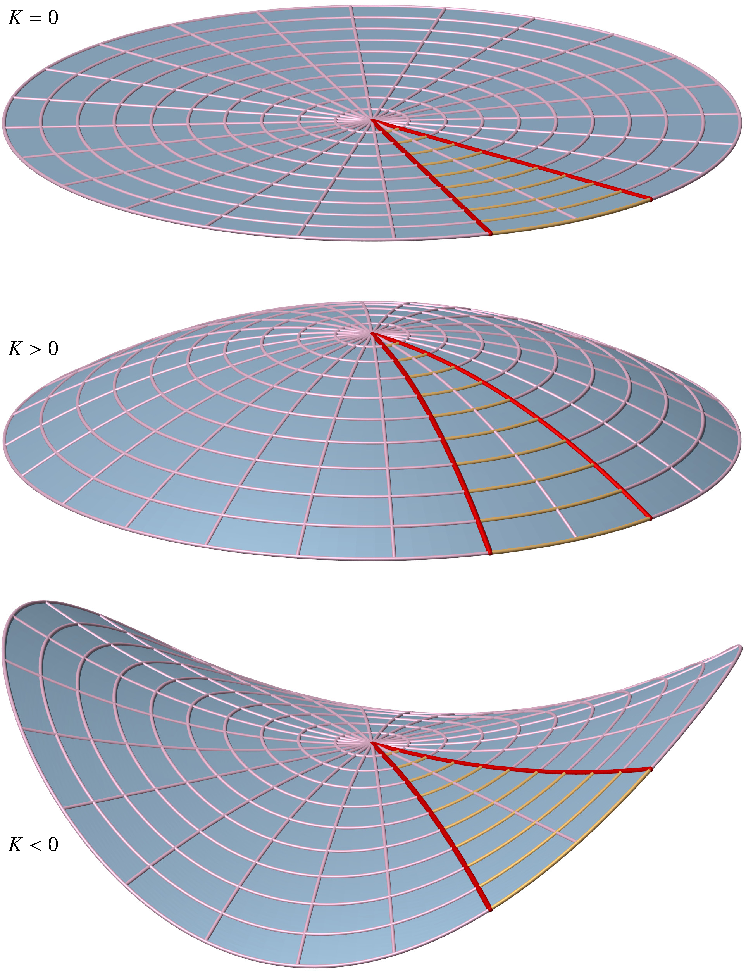
\includegraphics{chapters/110-kruemmung/images/kruemmung.pdf}
\caption{Die Schnittkrümmung bestimmt, wie schnell sich Geodäten
voneinander entfernen.
Der Abstand der Geodäten wächst linear mit dem Radius, wenn 
$K=0$ ist, der Abstand wächst schneller als linear für $K<0$ und
langsamer als linear für $K>0$.
\label{buch:kruemmung:fig:schnittkruemung}}
\end{figure}
